
% part 8
%Part 8: Deferred Poetry
\section{Отложенная поэзия\label{sec:part8}}

\subsection{Клиент 4.0}


%Now that we have know something about deferreds, we can rewrite our Twisted poetry client to use them. You can find client 4.0 in twisted-client-4/get-poetry.py.
Теперь, когда мы знаем что-то о deferred'ах, мы можем 
переписать наш Twisted поэтический клиент с их использованием. 
Вы можете найти клиент 4.0 в 
\href{http://github.com/jdavisp3/twisted-intro/blob/master/twisted-client-4/get-poetry.py}{twisted-client-4/get-poetry.py}.


%Our get_poetry function no longer needs callback or errback arguments. Instead, it returns a new deferred to which the user may attach callbacks and errbacks as needed.
Нашей функции get\_poetry не нужны больше аргументы callback или errback. 
Вместо этого она возвращает новый deferred, к которому пользователь 
может прикрепить необходимые callback'и и errback'и.

\begin{scriptsize}\begin{verbatim}
def get_poetry(host, port):
    """
    Download a poem from the given host and port. This function
    returns a Deferred which will be fired with the complete text of
    the poem or a Failure if the poem could not be downloaded.
    """
    d = defer.Deferred()
    from twisted.internet import reactor
    factory = PoetryClientFactory(d)
    reactor.connectTCP(host, port, factory)
    return d
\end{verbatim}\end{scriptsize}
%Our factory object is initialized with a deferred instead of a callback/errback pair. Once we have the poem, or we find out we couldn’t connect to the server, the deferred is fired with either a poem or a failure:
Наш объект  
\href{http://github.com/jdavisp3/twisted-intro/blob/master/twisted-client-4/get-poetry.py#L65}{factory}  
инициализируется с deferred'ом 
вместо пары  callback/errback. Как только мы получили поэму или 
обнаружили, что не можем присоединиться к серверу, deferred 
активизируется либо поэмой, либо ошибкой: 

\begin{scriptsize}\begin{verbatim}
class PoetryClientFactory(ClientFactory):

    protocol = PoetryProtocol

    def __init__(self, deferred):
        self.deferred = deferred

    def poem_finished(self, poem):
        if self.deferred is not None:
            d, self.deferred = self.deferred, None
            d.callback(poem)

    def clientConnectionFailed(self, connector, reason):
        if self.deferred is not None:
            d, self.deferred = self.deferred, None
            d.errback(reason)
\end{verbatim}\end{scriptsize}


%Notice the way we release our reference to the deferred after it is fired. This is a pattern found in several places in the Twisted source code and helps to ensure we do not fire the same deferred twice. It makes life a little easier for the Python garbage collector, too.
Заметьте способ, которым особобождается ссылка на 
deferred после активизации. Этот подход можно найти 
в нескольких местах исходных кодов Twisted, и этот способ  
помогает убедиться в том, что мы не активизируем один и тотже 
deferred дважды. Это также упрощает работу сборщика мусора в Python'е.


%Once again, there is no need to change the PoetryProtocol, it’s just fine as is. All that remains is to update the poetry_main function:
И снова, нет необходимости менять PoetryProtocol, он хорош 
как есть. Все, что осталось - обновить функцию poetry\_main: 

\begin{scriptsize}\begin{verbatim}
def poetry_main():
    addresses = parse_args()

    from twisted.internet import reactor

    poems = []
    errors = []

    def got_poem(poem):
        poems.append(poem)

    def poem_failed(err):
        print >>sys.stderr, 'Poem failed:', err
        errors.append(err)

    def poem_done(_):
        if len(poems) + len(errors) == len(addresses):
            reactor.stop()

    for address in addresses:
        host, port = address
        d = get_poetry(host, port)
        d.addCallbacks(got_poem, poem_failed)
        d.addBoth(poem_done)

    reactor.run()

    for poem in poems:
        print poem
\end{verbatim}\end{scriptsize}


%Notice how we take advantage of the chaining capabilities of the deferred to refactor the poem_done invocation out of our primary callback and errback.
Заметьте, что мы пользуемся способностью создавать цепочки 
вызовов в deferred'е для рефакторинга вызова poem\_done из 
нашего первоначального callback'а и errback'а.


%Because deferreds are used so much in Twisted code, it’s common practice to use the single-letter local variable d to hold the deferred you are currently working on. For longer term storage, like object attributes, the name “deferred” is often used.
Поскольку deferred'ы используются повсеместно в Twisted, 
то распостраненной практикой является использование 
однобуквенной локальной переменной d для хранения deferred, 
над которым вы сейчас работаете. Для длительного хранения, 
подобно атрибутам объекта, зачастую используется 
название "deferred".


\subsection{Обсуждение}

%With our new client the asynchronous version of get_poetry accepts the same information as our synchronous version, just the address of the poetry server. The synchronous version returns a poem, while the asynchronous version returns a deferred. Returning a deferred is typical of the asynchronous APIs in Twisted and programs written with Twisted, and this points to another way of conceptualizing deferreds:
С нашим новым клиентном асинхронная версия get\_poetry 
принимает ту же информация, что и асинхронная версия: 
только адрес поэтического сервера. Синхронная версия 
возвращает поэму, в то время как асинхронная версия 
возвращает deferred. Возвращать deferred - это типично для 
асинхронных API в Twisted и программах, написанных с 
помощью Twited, и это указывает на другой способ концептуализации deferred'ов:


%    A Deferred object represents an “asynchronous result” or a “result that has not yet come”.
Объект типа Deferred представляет "асинхронный результат" или 
"результат в пути".


%We can contrast these two styles of programming in Figure 13:
Мы можем сравнить эти два стиля программирования на рисунке \ref{fig:sync-async}:

% fig13
\begin{figure}[h]
\begin{center}
    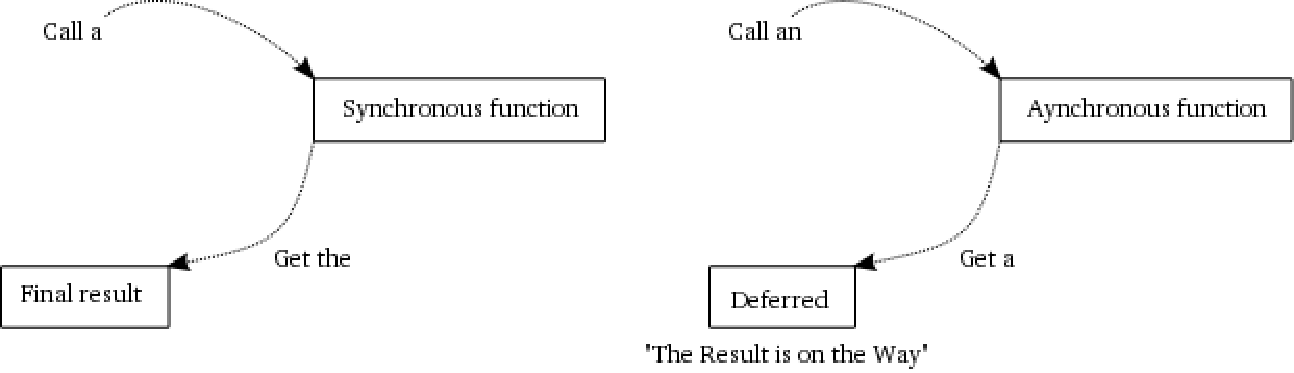
\includegraphics[width=0.8\textwidth]{images/sync-async.pdf}
    \caption{sync против async\label{fig:sync-async}}
\end{center}
\end{figure}


%By returning a deferred, an asynchronous API is giving this message to the user:
Возвращая deferred, асинхронное API сообщает следующее пользователю:

%    I’m an asynchronous function. Whatever you want me to do might not be done yet. But when it is done, I’ll fire the callback chain of this deferred with the result. On the other hand, if something goes wrong, I’ll fire the errback chain of this deferred instead.
    Я асинхронная функция. Требуемый результат еще не получен. 
Но, когда он будет получен, я активизирую цепочку callback'ов 
этого deferred'а с результатом. С другой стороны, если что-то пошло 
не так, то вместо этого я активизирую цепочку errback этого deferred'а.


%Of course, that function itself won’t literally fire the deferred, it has already returned. Rather, the function has set in motion a chain of events that will eventually result in the deferred being fired.
Конечно же, эта функция буквально сама не будет активизировать 
deferred, ее выполнение уже завершилось. Скорее, функция 
установила движение в цепочке событий, которые в конечном итоге 
приведут к активизации deferred'а.   


%So deferreds are a way of “time-shifting” the results of functions to accommodate the needs of the asynchronous model. And a deferred returned by a function is a notice that the function is asynchronous, the embodiment of the future result, and a promise that the result will be delivered.
Таким образом deferred'ы - способ "сдвига по времени" 
результатов функций для приспосабливания к нуждам 
асинхронной модели. И deferred, возвращенный функцией, - это 
знак того, что функция асинхронная, воплощение будущего 
результата и обещание того, что результат будет доставлен.


%It is possible for a synchronous function to return a deferred, so technically a deferred return value means the function is potentially asynchronous. We’ll see examples of synchronous functions returning deferreds in future Parts.
В случае синхронной функции возвратить deferred возможно, 
так что технически возврат deferred'а означает, что 
функция потенциально асинхронная. В следующих главах мы 
увидим примеры синхронных функций, возвращающих deferred'ы.


%Because the behavior of deferreds is well-defined and well-known (to folks with some experience programming with Twisted), by returning deferreds from your own APIs you are making it easier for other Twisted programmers to understand and use your code. Without deferreds, each Twisted program, or even each internal Twisted component, might have its own unique method for managing callbacks that you would have to learn in order to use it.
Поскольку поведение deferred'ов хорошо определено и 
хорошо изучено (для людей, имеющих некоторый опыт программирования 
с Twisted), возвращая deferred'ы из наших собственных API, 
вы упрощаете другим Twisted программистам понимание и использование 
вашего кода. Без deferred'ов, каждая Twisted программа или даже 
каждый Twisted компонент, может иметь свой собственный уникальный 
метод для управления callback'ми, которые вам надо изучить, для 
того, чтобы их использовать. 


%When You’re Using Deferreds, You’re Still Using Callbacks, and They’re Still Invoked by the Reactor
\subsection{Связь между deferred'ами, callback'ми, реактором}


%When first learning Twisted, it is a common mistake to attribute more functionality to deferreds than they actually have. Specifically, it is often assumed that adding a function to a deferred’s chain automatically makes that function asynchronous. This might lead you to think you could use, say, os.system with Twisted by adding it to a deferred with addCallback.
При первом изучении Twisted, общераспостраненной ошибкой 
присваивать большую функциональность deferred'ам, нежели 
они в действительности имеют. Особенно, зачастую предполагается, 
что добавление функции в цепочку deferred'а, автоматически 
делает эту функцию асинхронной. Это могло бы навести на мысль, 
что вы могли бы использовать, скажем, os.system с Twisted 
добавляя его в deferred с помощью addCallback.


%I think this mistake is caused by trying to learn Twisted without first learning the asynchronous model. Since typical Twisted code uses lots of deferreds and only occasionally refers to the reactor, it can appear that deferreds are doing all the work. If you have read this introduction from the beginning, it should be clear this is far from the case. Although Twisted is composed of many parts that work together, the primary responsibility for implementing the asynchronous model falls to the reactor. Deferreds are a useful abstraction, but we wrote several versions of our Twisted client without using them in any way.
Думается, что эта ошибка вызвана попыткой изучить 
Twisted без первоначального изучения асинхронной модели. 
Поскольку типичный Twsisted код использует много deferred'ов, 
и только иногда ссылается на reactor, может показаться, что 
deferred'ы делают всю работу. Если вы читали введение с 
самого начала, то должно быть ясно, что это далеко от реальности. 
Хотя Twisted составлен из многих частей, которые работают вместе, 
первоначальная ответственность за реализацию асинхронной 
модели ложится на reactor. Deferred'ы - полезная абстракция, но 
мы написали несколько версий нашего поэтического Twisted 
клинта без их использования.


%Let’s look at a stack trace at the point when our first callback is invoked. Run the example program in twisted-client-4/get-poetry-stack.py with the address of a running poetry server. You should get some output like this:
Давайте посмотрим на stack trace в месте, когда вызывается 
наш первый callback. Запустите пример программы из 
\href{http://github.com/jdavisp3/twisted-intro/blob/master/twisted-client-4/get-poetry-stack.py}{twisted-client-4/get-poetry-stack.py} с адресом запущенного поэтического сервера. 
Вы получите следующий вывод:

\begin{scriptsize}\begin{verbatim}
  File "twisted-client-4/get-poetry-stack.py", line 129, in
    poetry_main()
  File "twisted-client-4/get-poetry-stack.py", line 122, in poetry_main
    reactor.run()

  ... # some more Twisted function calls

    protocol.connectionLost(reason)
  File "twisted-client-4/get-poetry-stack.py", line 59, in connectionLost
    self.poemReceived(self.poem)
  File "twisted-client-4/get-poetry-stack.py", line 62, in poemReceived
    self.factory.poem_finished(poem)
  File "twisted-client-4/get-poetry-stack.py", line 75, in poem_finished
    d.callback(poem) # here's where we fire the deferred

  ... # some more methods on Deferreds

  File "twisted-client-4/get-poetry-stack.py", line 105, in got_poem
    traceback.print_stack()
\end{verbatim}\end{scriptsize}

%That’s pretty similar to the stack trace we created for client 2.0. We can visualize the latest trace in Figure 14:
Это очень похоже на stack trace, который мы создали для клиента 2.0. 
Визуализируем последний trace на рисунке \ref{fig:reactor-deferred-callback}:

% fig14
\begin{figure}[h]
\begin{center}
    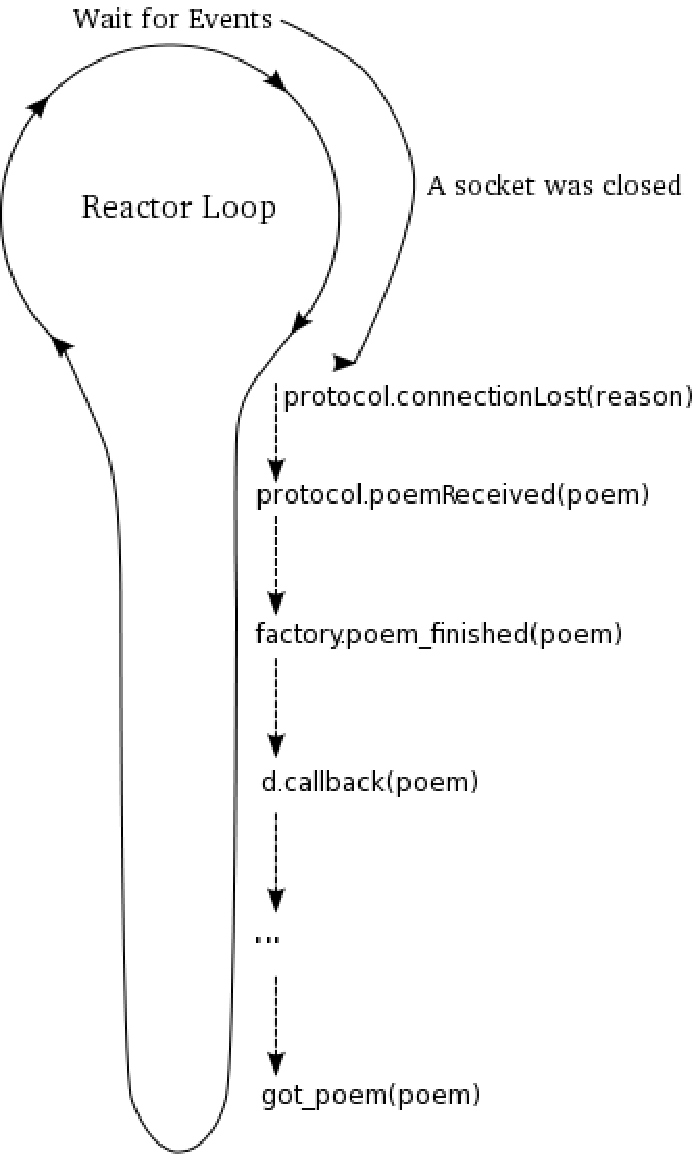
\includegraphics[height=0.5\textheight]{images/reactor-deferred-callback.pdf}
    \caption{callback с использованием deferred'а\label{fig:reactor-deferred-callback}}
\end{center}
\end{figure}

%Again, this is similar to our previous Twisted clients, though the visual representation is starting to become vaguely disturbing. We probably won’t be showing any more of these, for the sake of the children. One wrinkle not reflected in the figure: the callback chain above doesn’t return control to the reactor until the second callback in the deferred (poem_done) is invoked, which happens right after the first callback (got_poem) returns.
И снова, это подобно нашим предыдущим Twisted клиентам, 
хотя визуальное представление становится неясным. 
Одно замечание, не касающееся рисунка: цепочка callback'ов 
выше не возвратит управление реактору до того, как не 
вызовется второй callback в deferred'е (poem\_done), 
что произойдет сразу после возврата из первого callback'а (got\_poem). 


%There’s one more difference with our new stack trace. The line separating “Twisted code” from “our code” is a little fuzzier, since the methods on deferreds are really Twisted code. This interleaving of Twisted and user code in a callback chain is common in larger Twisted programs which make extensive use of other Twisted abstractions.
Есть еще одно отличие в нашем новом stack trace'е. Граница, 
разделяющая "код Twisted" от "нашего кода" немного размыта, 
поскольку deferred'ы - это в реальности Twisted код. Это чередование 
Twisted и пользовательского кода в callback-цепочке является 
общепринятым в большинстве программ, написанных с использованием 
Twisted, активно использующих различные Twisted абстракции.
 

%By using a deferred we’ve added a few more steps in the callback chain that starts in the Twisted reactor, but we haven’t changed the fundamental mechanics of the asynchronous model. Recall these facts about callback programming:
Используя deferred, мы добавили несколько шагов 
в callback-цепочку, которая начинается в реакторе Twisted, 
но мы не поменяли фундаментальных механизмов асинхронной модели. 
Вспомним факты о программировании с использованием callback'ов:

\begin{enumerate}

%   1. Only one callback runs at a time.
\item Только один callback выполняется в один момент.

%   2. When the reactor is running our callbacks are not.
\item Когда выполняется reactor, наши callback'и - нет. 

%   3. And vice-versa.
\item И наоборот.

%   4. If our callback blocks then the whole program blocks.
\item Если наш callback блокируется, то вся программа блокируется.

\end{enumerate}


%Attaching a callback to a deferred doesn’t change these facts in any way. In particular, a callback that blocks will still block if it’s attached to a deferred. So that deferred will block when it is fired (d.callback), and thus Twisted will block. And we conclude:
Присоединение callback'а к deferred'у никак не меняет эти факты. 
В особенности, callback, который блокируется, все еще будет блокироваться, 
даже после присоединения к deferred'у. Поэтому deferred заблокируется при 
активизации (d.callback), поэтому все остальное тоже заблокируется. Поэтому мы заключаем, что:   


%    Deferreds are a solution (a particular one invented by the Twisted developers) to the problem of managing callbacks. They are neither a way of avoiding callbacks nor a way to turn blocking callbacks into non-blocking callbacks.
    Deferred'ы - решение (разработанное разработчиками Twisted) 
проблемы управления callback'ми. Они не являются ни способом 
мзбежать callback'ов, ни способом превратить блокирующиеся 
callback'и в неблокирующиеся. 


%We can confirm the last point by constructing a deferred with a blocking callback. Consider the example code in twisted-deferred/defer-block.py. The second callback blocks using the time.sleep function. If you run that script and examine the order of the print statements, it will be clear that a blocking callback also blocks inside a deferred.
Мы можем подтвердить наш последний вывод созданием deferred'а 
с блокирующм callback'ом. Рассмотрим пример кода в 
\href{http://github.com/jdavisp3/twisted-intro/blob/master/twisted-deferred/defer-block.py}{twisted-deferred/defer-block.py}. 
Второй callback блокируется, используя функцию time.sleep. Если вы запустите 
этот скрипт и проверите порядок операторов print, то будет ясно, что 
блокирующийся callback также блокируется, находясь внутри deferred'а.


\subsection{Резюме}

%By returning a Deferred, a function tells the user “I’m asynchronous” and provides a mechanism (add your callbacks and errbacks here!) to obtain the asynchronous result when it arrives. Deferreds are used extensively throughout the Twisted codebase and as you explore Twisted’s APIs you are bound to keep encountering them. So it will pay to become familiar with deferreds and comfortable in their use.
Возвращая Deferred, функция говорит пользователю "Я асинхронная" и 
обеспечивает механизм (добавь здесь callback'и и errback'и!) 
получения асинхронного результата в момент, когда он прибудет. 
Deferred'ы повсеместно используются в Twisted, поэтому с ними 
надо ознакомиться и знать, как применять.


%Client 4.0 is the first version of our Twisted poetry client that’s truly written in the “Twisted style”, using a deferred as the return value of an asynchronous function call. There are a few more Twisted APIs we could use to make it a little cleaner, but I think it represents a pretty good example of how simple Twisted programs are written, at least on the client side. Eventually we’ll re-write our poetry server using Twisted, too.
Клиент 4.0 - первая версия нашего Twisted поэтического 
клиента, которая действительно написана в стиле Twisted, 
используя deferred'ы в качестве возвращаемых значений 
асинхронного вызова функций. Есть еще другие Twisted API, 
которые мы могли бы использовать для того, чтобы сделать код 
понятнее, но я думаю, что он представляет достаточно 
хороший пример того, как написать простые Twisted программы, 
по меньшей мере на стороне клиента. В конечном итоге, мы 
также перепишем наш поэтический сервер с использованием Twisted. 


%But we’re not quite finished with deferreds. For a relatively short piece of code, the Deferred class provides a surprising number of features. We’ll talk about some more of those features, and their motivation, in Part 9.
Но мы еще не окончили с deferred'ми. Для относительно 
небольшого куска кода, класс Deferred предоставляется 
удивительный ряд возможностей. Мы остановимся подоробнее 
на некоторых из этих возможностях и их мотифированности в 
следующей главе.


\subsection{Упражнения}

\begin{enumerate}

%   1. Update client 4.0 to timeout if the poem isn’t received after a given period of time. Fire the deferred’s errback with a custom exception in that case. Don’t forget to close the connection when you do.
\item Обновите клиент 4.0 для установки timeout'а, в случае, если 
поэмы не была получена за заданный период времени. Активизируйте в этом 
случае errback deferred'а, используя пользовательское исключение. Не 
забудьте закрыть соединение.

%   2. Update client 4.0 to print out the appropriate server address when a poem download fails, so the user can tell which server is the culprit. Don’t forget you can add extra positional- and keyword-arguments when you attach callbacks and errbacks.
\item Обновите клиент 4.1 для того, чтобы распечатать 
соответствующий адрес сервера при ошибки скачивания поэмы так, 
чтобы пользователь смог сказать какой сервер виновник. Не забудьте, 
что вы можете добавить дополнительные позиционные и keyword-аргументы, 
при присоединении callback'ов и errback'ов.

\end{enumerate}

